\section{Auswertung}
\label{sec:auswertung}
	Im Folgenden werden alle Schwingungsdauertn $T$ "uber drei Perioden gemessen und gemittelt.
	Zudem werden jeweils 10 Messungen vorgenommen und ein Mittelwert $\overline{T}$ mit der Standardabweichung $\sigma$ gebildet.
	Bei einer Anzahl von $n$ Stichproben gilt

	\begin{eqnarray}
		\overline{T} & = & \frac{1}{n} \sum_{i = 1}^n{T_i} \nonumber \\
		%\sigma_T = \sqrt{\frac{1}{n-1}\sum_{i = 1}^n {(T_i - \overline{T})^2}} \,.
		\Delta T & = & \left(\frac{1}{n-1}\sum_{i = 1}^n {(T_i - \overline{T})^2}\right)^{\frac{1}{2}} \,. \nonumber
	\end{eqnarray}

	Der Ablesefehler bei L"angenbestimmung liegt bei allen Werten bei $\Delta x = \SI{.5}{\milli \meter}$.

	\subsection{Bestimmung der Winkelrichtgr"o"se $D$}
	\label{subsec:winkelrichtgroesse}
		Zun"achst muss die Winkelrichtgr"o"se $D$ aus Gleichung \eqref{eqn:richtgroesse} bestimmt werden.
		Die folgende Tabelle zeigt die Messwerte. F"ur die Winkelrichtgr"o"se erh"alt man damit

		\begin{equation*}
			D = \SI{.348 (75)}{\milli \newton \meter} \,.
		\end{equation*}

		\begin{table}[h!]
			\begin{center}
				\label{tabelle:winkelrichtgroesse}
				\caption{Messwerte f"ur die Bestimmung der Winkelrichtgr"o"se $D$}
				\begin{tabular}{|c|c|c|c||c|c|c|c|}
					\hline
					$r [\SI{}{\centi \meter}]$ & $\varphi [\SI{}{\degree}]$ &  $F [\SI{}{\milli \newton}]$ & $D [\SI{}{\milli \newton \meter}]$ & $r [\SI{}{\centi \meter}]$ & $\varphi [\SI{}{\degree}]$ &  $F [\SI{}{\milli \newton}]$ & $D [\SI{}{\milli \newton \meter}]$\\
					\hline 
					\hline
					20	&	 10	&	10 & 2,00 & 20	&	 60	&	33 & 3,63 \\
20	&	 20	&	16 & 2,50 & 20	&	 71	&	35 & 4,05 \\
20	&	 30	&	20 & 3,00 & 20	&	 80	&	38 & 4,21 \\
20	&	 41	&	23 & 3,56 & 20	&	 90	&	44 & 4,09 \\
20	&	 50	&	27 & 3,70 & 20	&	101	&	50 & 4,04 \\





					\hline 
				\end{tabular}
			\end{center}
		\end{table}

	\subsection{Bestimmung des Eigentr"agheitsmomentes $I_\mathrm{D}$ der Drehachse}
	\label{subsec:eigentraegheitsmoment}
		Um den Einfluss des Eigentr"agheitsmomentes $I_\mathrm{D}$ der Apparatur auf die Messwerte zu bestimmen, muss dieses gemessen werden.
		Hierbei werden zwei Gewichte der Masse $m$ im gleichen Abstand $a$ zur Drehachse an einem Metallstab der Masse $M$ und der L"ange $l$ angebracht.
		Das Gesamttr"agheitsmoment des Systems wird dann durch

		\begin{equation}
			I = I_\mathrm{D} + I_\mathrm{Stange} + 2 I_\mathrm{m} \, \label{eqn:gesamtmoment}
		\end{equation}

		beschrieben, wobei das Tr"agheitsmoment der Stange durch $I_\mathrm{stange}$ gegeben ist und $I_\mathrm{m}$ das Tr"agheitsmoment eines Gewichtes unter Ber"ucksichtigung des Steinerschen Satzes bezeichnen.
		Hierbei kann n"aherungsweise angenommen werden, dass f"ur gegen $a$ kleine Radien $r$ und geringe H"ohen $h$, der zylindrischen Gewichten, gilt:

		\begin{equation*}
			I_\mathrm{m} = \frac{1}{4}mr^2 + \frac{1}{12}mh^2 + ma^2 \approx ma^2 \,.
		\end{equation*}

		Die Gleichung \eqref{eqn:schwingungsdauer} und \eqref{eqn:gesamtmoment} liefern dann den Zusammenhang

		\begin{eqnarray*}
			T^2 & = & \frac{4 \pi^2}{D} \left(I_\mathrm{D} + I_\mathrm{Stange} + 2ma^2 \right) = \frac{4 \pi^2}{D} \left(B  + 2ma^2 \right) \,, \\
			\Rightarrow \quad I_\mathrm{D} & = & B - I_\mathrm{Stange} \,.
		\end{eqnarray*}

		Das Eigentr"agheitsmoment $I_\mathrm{D}$ kann also durch Messung von $T$ und $a$ mit einer Ausgleichsrechnung bestimmt werden. Es gilt au"serdem

		\begin{eqnarray*}
			M = \SI{96.28}{\gram} &,& l = \SI{60}{\centi \meter} \\
			\Rightarrow \quad I_\mathrm{Stange} & = & \frac{1}{12} M l^2 = \SI{2.89}{\gram \meter \squared} \,, \\
			\Delta I_\mathrm{D} & = & \sqrt{\left(\Delta B\right)^2 + \left(\frac{1}{6}Ml \Delta l \right)^2} \,.
		\end{eqnarray*}

		Die Ausgleichsrechnung durch \emph{python} liefert

		\begin{eqnarray*}
			B & = & \SI{-.017 (3)}{\gram \meter \squared} \\
			\Rightarrow \quad I_\mathrm{D} & = & \SI{-2.91 (5)}{\gram \meter \squared} \,.
		\end{eqnarray*}

		Ein negatives Tr"agheitsmoment ergibt physikalisch keinen Sinn und wird daher im Verlauf nicht mehr genutzt. Fehlerquellen werden in der Diskussion behandelt

		Die zur Berechnung genutzten Daten werden in folgender Tabelle aufgef"uhrt.

		\begin{table}[h!]
			\begin{center}
				\label{tabelle:winkelrichtgroesse}
				\caption{Messwerte f"ur die Bestimmung des Eigentr"agheitsmomentes $I_\mathrm{D}$}
				\begin{tabular}{|c|c||c|c|}
					\hline
					$a [\SI{}{\centi \meter}]$ & $T [\SI{}{\second}]$ & $a [\SI{}{\centi \meter}]$ & $T [\SI{}{\second}]$\\
					\hline 
					\hline
					26	&	20,16	& 16	&	13,12\\
26	&	20,13	& 16	&	13,16\\
24	&	18,60	& 14	&	11,75\\
24	&	18,50	& 14	&	11,72\\
22	&	17,18	& 12	&	10,53\\
22	&	17,22	& 12	&	10,53\\
20	&	15,78	& 10	&	09,34\\
20	&	15,88	& 10	&	09,37\\
18	&	14,69	& 08	&	08,31\\
18	&	14,64	& 08	&	08,25\\
					\hline 
				\end{tabular}
			\end{center}
		\end{table}

		\subsection{Bestimmung der Tr"agheitsmomente $I_\mathrm{k}$ verschiedener K"orper}
		\label{subsec:versch_momente}
			Schlie"slich werden die Tr"agheitsmomente $I_\mathrm{k}$ f"ur $k$ verschiedene K"orper bestimmt.
			Dabei handelt es sich um eine Holzkugel, einen Messingzylinder, sowie eine Holzpuppe, die in zwei verschiedenen K"orperhaltungen eingespannt wird.

			Aus der Periodendauer wird dann gem"a"s Gleichung \eqref{eqn:schwingungsdauer} das Tr"agheitsmoment berechnet.
			Es gilt

			\begin{eqnarray*}
				I & = & \frac{T^2 D}{4 \pi^2} \,, \\
				\Delta I & = & \sqrt{\left(\frac{TD}{2 \pi^2} \Delta T\right)^2 + \left(\frac{T^2}{4 \pi^2} \Delta D\right)^2} \,.
			\end{eqnarray*}

			Die experimentellen Daten werden zudem mit den theoretischen Werten verglichen, um ihre Aussagekraft zu beurteilen.
			Hierzu wird jeweils der relative Unterschied $\delta_\mathrm{k}$ in Prozent angegeben.

			\clearpage
			\subsubsection{Die gro"se Holzkugel}
			\label{subsubsec:holzkugel}
				\begin{figure}[htbp]
					
					\begin{minipage}[t]{8cm}
						\vspace{0pt}
						Das Tr"agheitsmoment $I_\mathrm{1, theorie}$ der Holzkugel berechnet sich nach

						\begin{eqnarray*}
							I_\mathrm{1, theorie} & = & \frac{2}{5}mr^2 \,, \\
							\Delta I_\mathrm{1, theorie} & = & \frac{2}{5} \sqrt{ \left(r^2 \Delta m\right)^2 + \left( 2 mr \Delta r\right)^2} \,.
						\end{eqnarray*}

						Mit den gemessenen Werten f"ur die Masse $m$ und den Radius $r$ folgt

						\begin{eqnarray*}
							m & = & \SI{1168.4 (1)}{\gram} \,, \\
							r & = & \SI{7.35 (5)}{\centi \meter} \,, \\
							\Rightarrow \quad I_\mathrm{1, theorie} & = & \SI{2.53 (34)}{\gram \meter \squared} \,.
						\end{eqnarray*}

						Folgende Tabelle beinhaltet die Messdaten zur experimentellen Bestimmung:
					\end{minipage}
					\hfill
					\begin{minipage}[t]{5cm}
						\vspace{0pt}
						\centering
						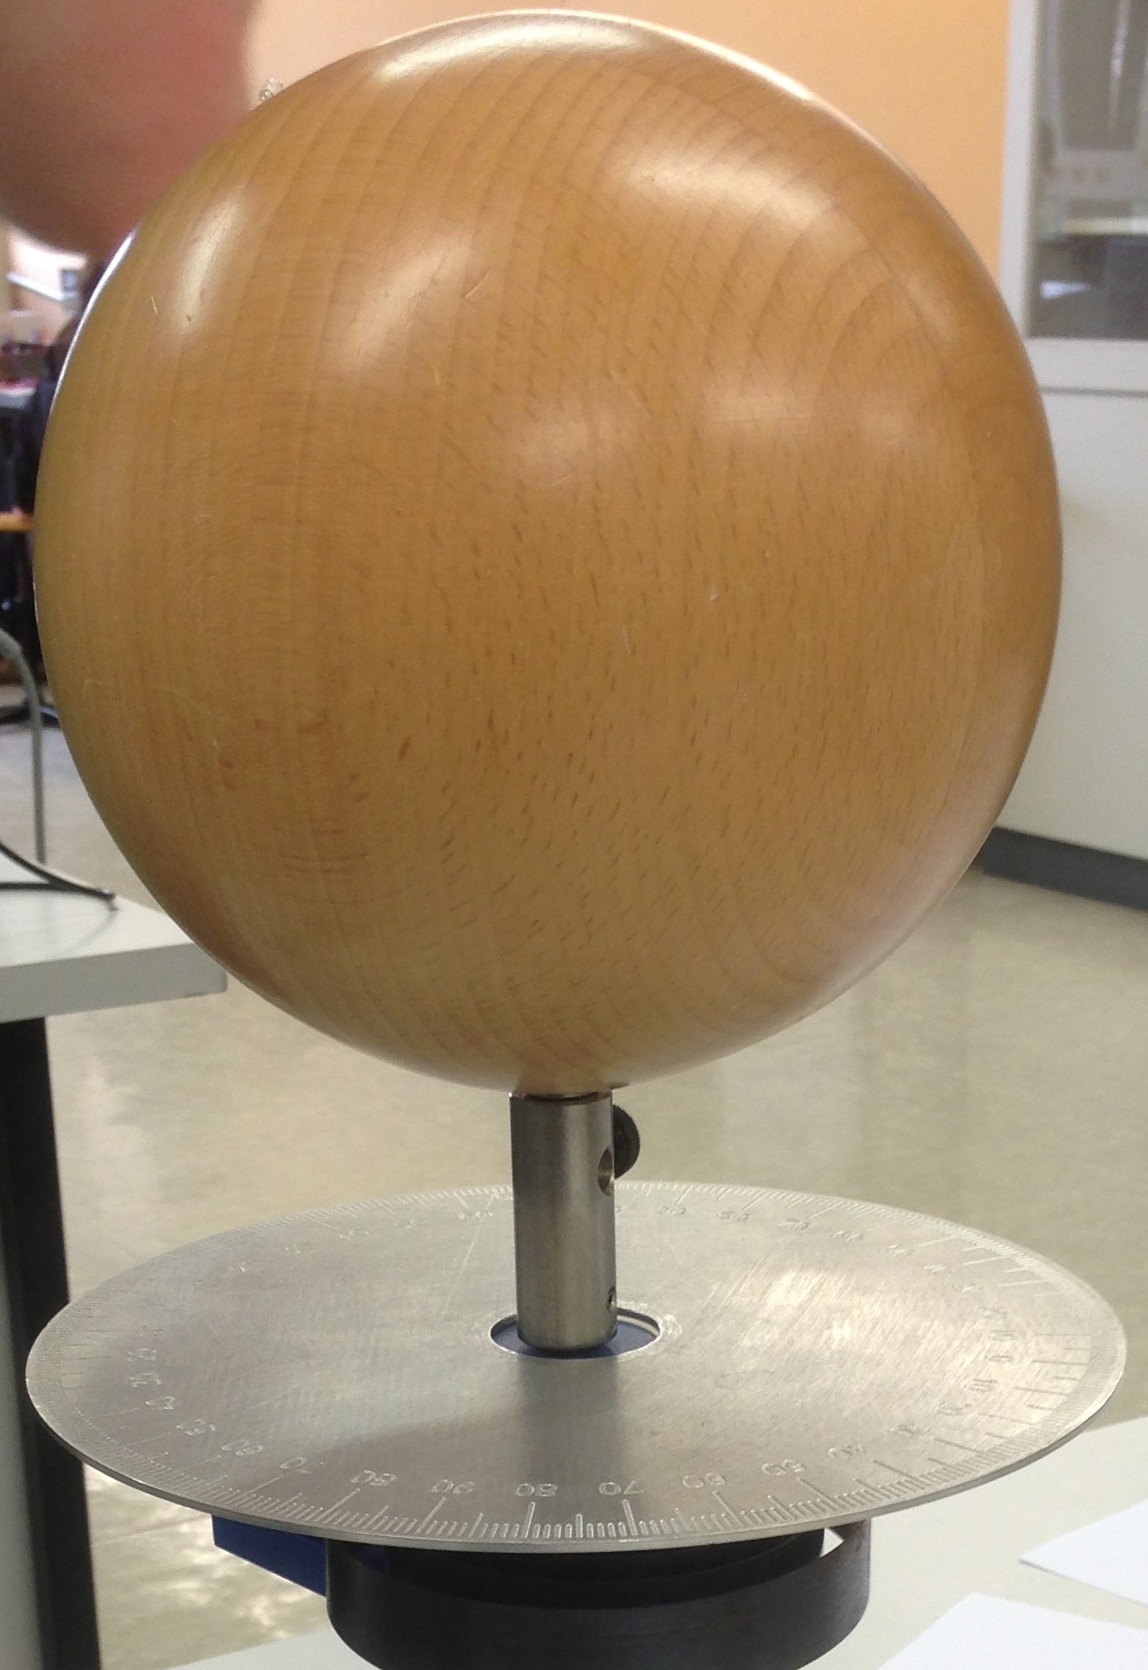
\includegraphics[width = 5cm]{img/kugel.jpg}
						\caption{Kugelk"orper}
						\label{fig:kugel}
					\end{minipage}
				\end{figure}

				\begin{table}[h!]
					\begin{center}
						\label{tabelle:kugel}
						\caption{Messwerte f"ur die Bestimmung des Tr"agheitsmomentes $I_\mathrm{1, exp}$ der Holzkugel}
						\begin{tabular}{|c||c||c|}
							\hline
							$T [\SI{}{\second}]$ & $T [\SI{}{\second}]$ & $T [\SI{}{\second}]$ \\
							\hline 
							\hline
							1,82 & 1,84 & 1,84 \\
1,82 & 1,87 & 1,82 \\
1,82 & 1,83 & 1,86 \\
1,85 & -    & -    \\











							\hline 
						\end{tabular}
					\end{center}
				\end{table}

				Die Messwerte liefern mit Gleichung \eqref{eqn:schwingungsdauer}

				\begin{eqnarray*}
					I_\mathrm{1, exp} & = & \SI{1.71 (3)}{\gram \meter \squared} \,, \\
					\delta_1 & = & \SI{32.4}{\percent} \,.
				\end{eqnarray*}

			\clearpage
			\subsubsection{Der Messingzylinder}
			\label{subsubsec:holzkugel}
				\begin{figure}[htbp]
					
					\begin{minipage}[t]{8cm}
						\vspace{0pt}
						Das Tr"agheitsmoment $I_\mathrm{2, theorie}$ des Zylinders berechnet sich unabh"angig von der H"ohe nach

						\begin{eqnarray*}
							I_\mathrm{2, theorie} & = & \frac{1}{2}mr^2 \,, \\
							\Delta I_\mathrm{2, theorie} & = & \frac{1}{2} \sqrt{ \left(r^2 \Delta m\right)^2 + \left( 2 mr \Delta r\right)^2} \,.
						\end{eqnarray*}

						Mit den gemessenen Werten f"ur die Masse $m$ und den Radius $r$ folgt

						\begin{eqnarray*}
							m & = & \SI{1436.0 (1)}{\gram} \,, \\
							r & = & \SI{4.25 (5)}{\centi \meter} \,, \\
							\Rightarrow \quad I_\mathrm{2, theorie} & = & \SI{1.30 (3)}{\gram \meter \squared} \,.
						\end{eqnarray*}

						Folgende Tabelle beinhaltet die Messdaten zur experimentellen Bestimmung:
					\end{minipage}
					\hfill
					\begin{minipage}[t]{5cm}
						\vspace{0pt}
						\centering
						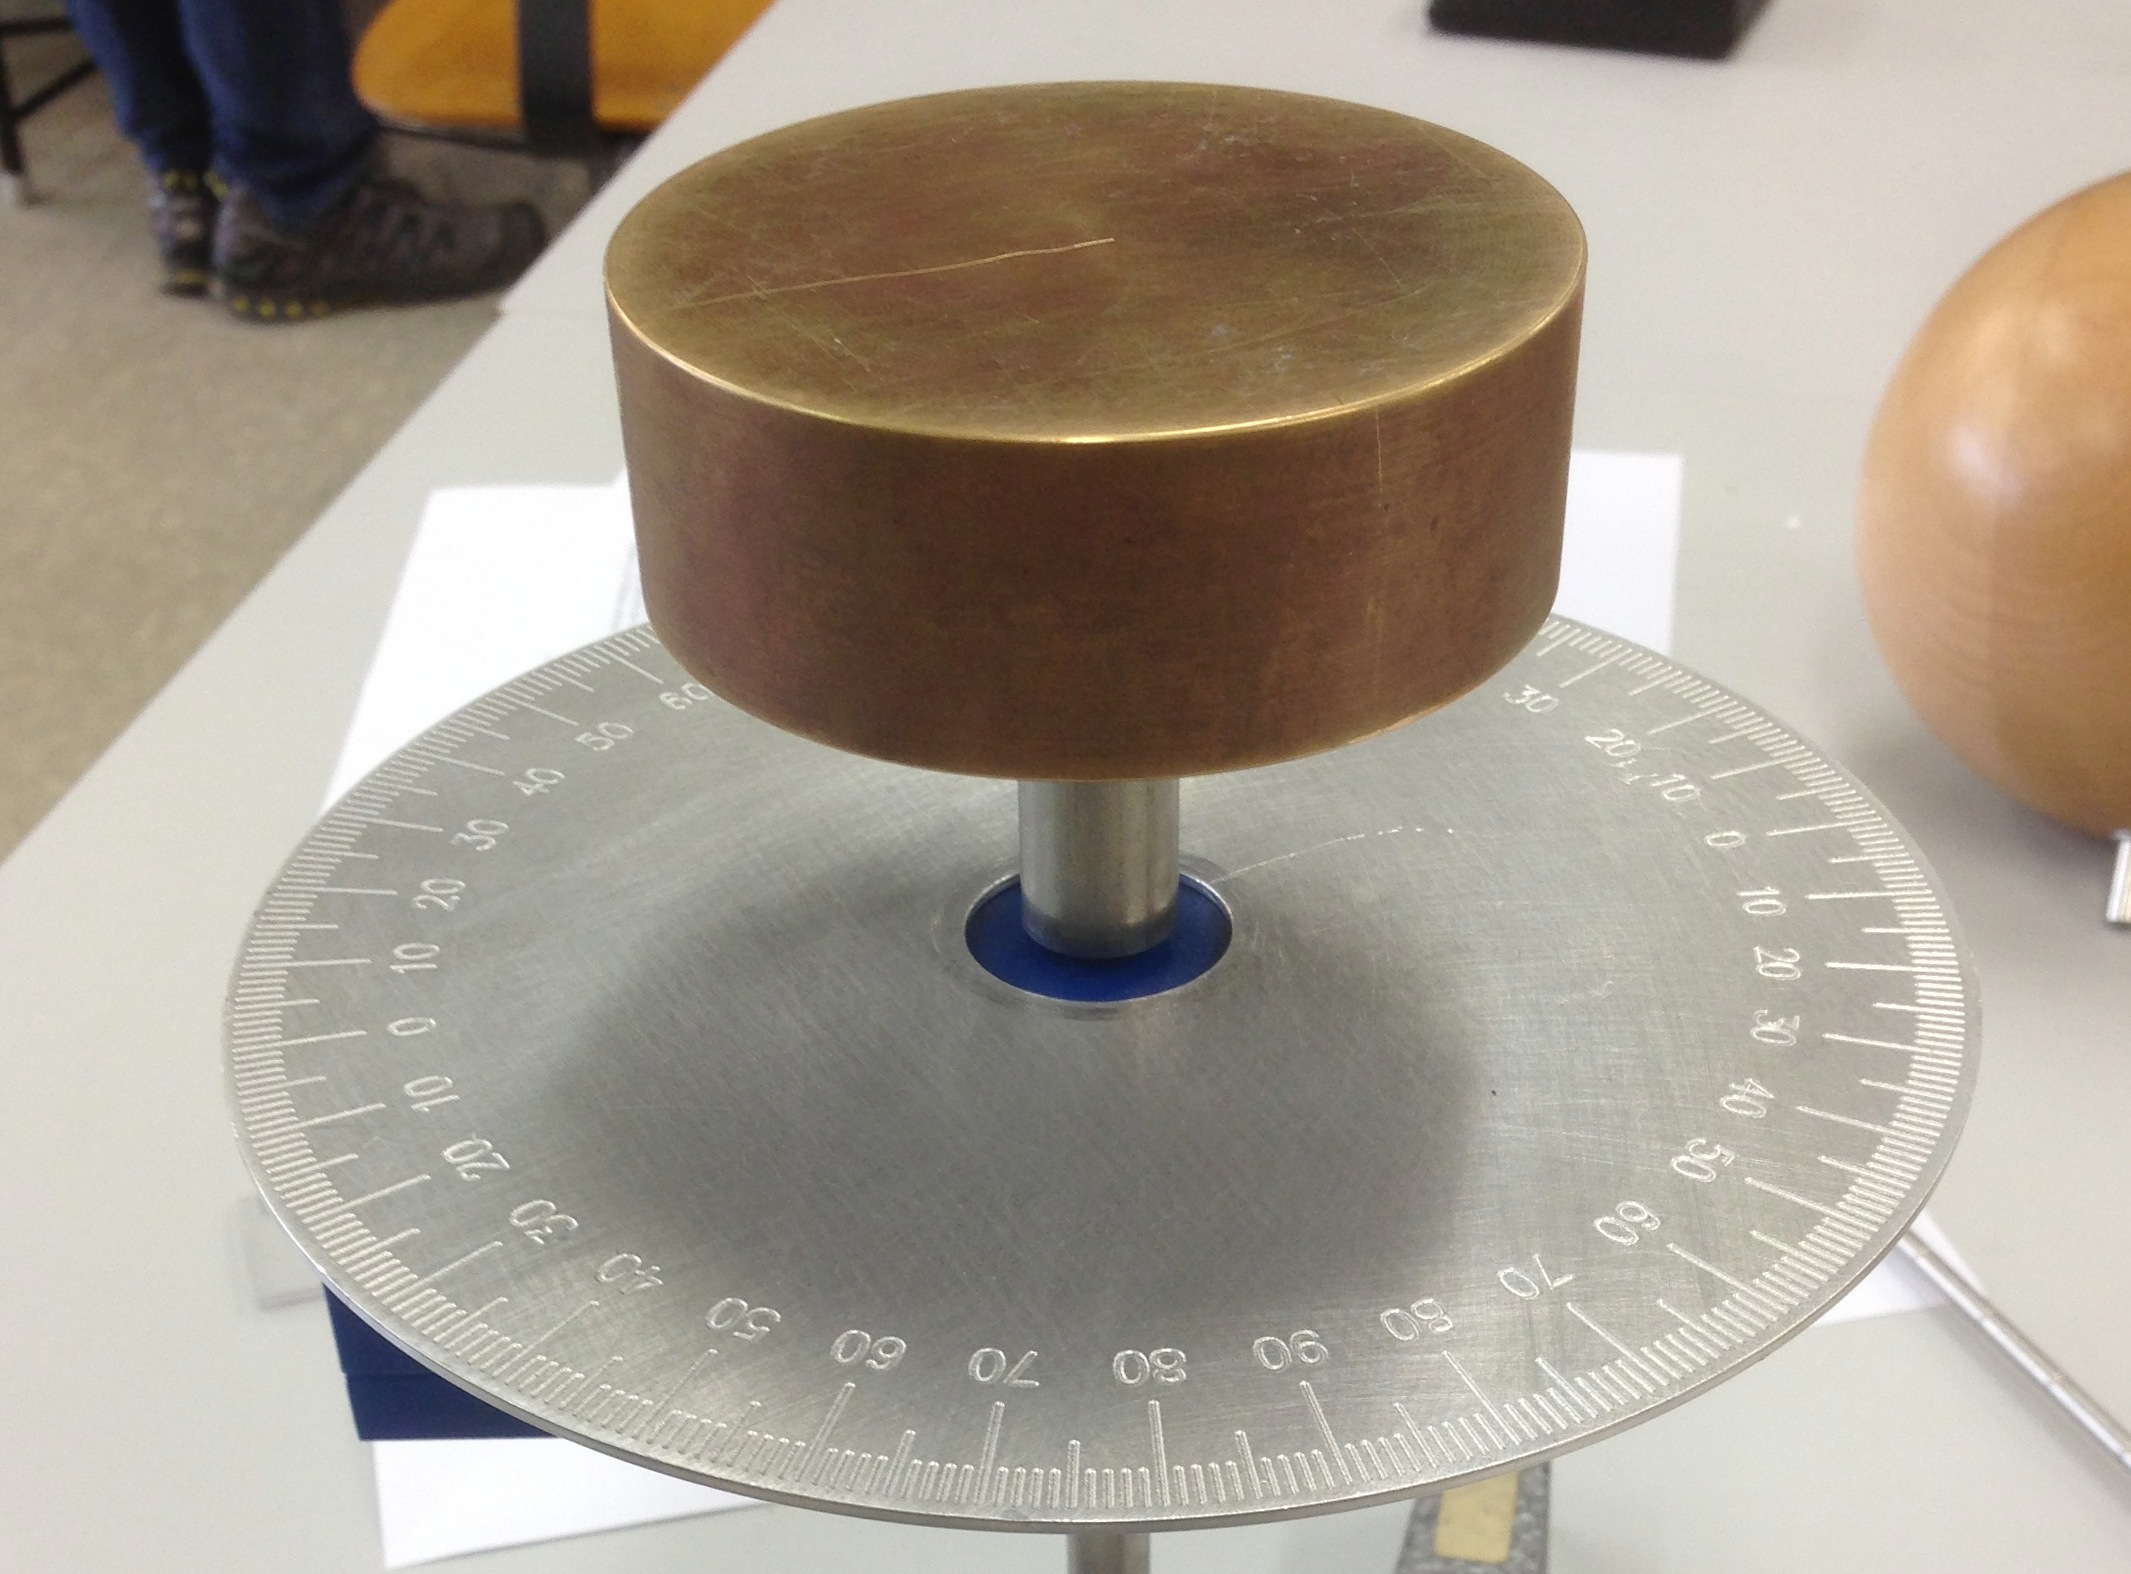
\includegraphics[width = 5cm]{img/messing.jpg}
						\caption{Messingzylinder}
						\label{fig:zylinder}
					\end{minipage}
				\end{figure}

				\begin{table}[h!]
					\begin{center}
						\label{tabelle:kugel}
						\caption{Messwerte f"ur die Bestimmung des Tr"agheitsmomentes $I_\mathrm{2, exp}$ des Messingzylinders}
						\begin{tabular}{|c||c||c|}
							\hline
							$T [\SI{}{\second}]$ & $T [\SI{}{\second}]$ & $T [\SI{}{\second}]$ \\
							\hline 
							\hline
							1,34 & 1,35 & 1,32 \\
1,35 & 1,34 & 1,32 \\
1,31 & 1,32 & 1,33 \\
1,30 & -    & -    \\











							\hline 
						\end{tabular}
					\end{center}
				\end{table}

				Die Messwerte liefern mit Gleichung \eqref{eqn:schwingungsdauer}

				\begin{eqnarray*}
					I_\mathrm{2, exp} & = & \SI{.89 (2)}{\gram \meter \squared} \,, \\
					\delta_2 & = & \SI{31.5}{\percent} \,.
				\end{eqnarray*}

			\clearpage
			\subsubsection{Puppe}
			\label{subsubsec:puppe}
				

